\documentclass{report}
\usepackage{tikz}
\usetikzlibrary{positioning,shapes,arrows}
\usepackage{xcolor,colortbl}
\usepackage{caption}
\usepackage{subcaption}
\usepackage{amsmath}
\usepackage{amssymb}
\usepackage{hyperref}

\setlength{\parindent}{0cm}

\title{Artificial Intelligence Notes}
\author{Patrick Oliver GLAUNER \\
	\texttt{patrick.oliver.glauner@gmail.com}}

\date{\today}

\newtheorem{definition}{Definition}[section]

\newcommand\independent{\protect\mathpalette{\protect\independenT}{\perp}}
\def\independenT#1#2{\mathrel{\rlap{$#1#2$}\mkern2mu{#1#2}}}

\begin{document}

\maketitle

\tableofcontents

\begin{abstract}
{\em Artificial Intelligence (AI)} is a versatile field and there are many different definitions for it. My favorite definition is:
\begin{flushright}
{\em "AI is the science of knowing what to do when you don't know what to do". (Peter Norvig)}\footnote{\url{https://www.youtube.com/watch?v=rtmQ3xlt-4A4m45}}
\end{flushright}
~\\
This document aggregates definitions and findings that are related to AI with a strong focus on {\em Machine Learning}. It will continuously be updated in the future.
~\\~\\
Most of the content is based on:
\begin{itemize}
\item Stuart Russell and Peter Norvig. {\em Artificial Intelligence: A Modern Approach}. Third edition.\footnote{\url{http://aima.cs.berkeley.edu/}}
\item Andrew Ng. {\em Machine Learning}. Stanford University.\footnote{\url{https://www.coursera.org/course/ml}}
\end{itemize}

~\\~\\~\\~\\
\begin{flushright}
Patrick GLAUNER
\end{flushright}

\end{abstract}


\chapter{General}
\section{Terminology}
\subsection{Intelligent agents}
An {\bf agent} operates autonomously. A {\bf rational agent} acts to achieve the best outcome or expected outcome if there is uncertainty. An {\bf agent program} implements the {\bf agent function} which maps perceptions to actions.

\subsection{Task environments}
{\bf Single vs. multi agent}: the agent is the only one. {\bf Fully observable} vs. {\bf partially observable}: the agent's sensors perceive the complete state of the relevant environment at each point in time. {\bf Deterministic} vs. {\bf stochastic}: the agent's state and action uniquely determine the next state. {\bf Discrete} vs. {\bf continuous}: finite amount of states, actions and outcomes. {\bf Benign} vs. {\bf adversarial}: there is no opponent. {\bf Known vs. unknown}: the agent's knowledge about the "law of physics" of the environment, the outcomes (or probabilities) for all actions are given.



\chapter{Probabilities}
\section{Introduction} 

\begin{definition}[Complement]
$P(\neg A) = 1 - P(A)$
\end{definition}

\begin{definition}[Inclusion-exclusion principle]
$P(A\vee B) =P(A) + P(B) - P(A,B)$
\end{definition}


\section{Independence}

\begin{figure}[h!]
\centering
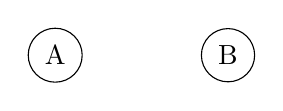
\begin{tikzpicture}[
  node distance=1cm and 1cm,
  mynode/.style={draw,circle,align=center}
]
\node[mynode] (A) {A};
\node[mynode, right=1.5cm of A] (B) {B};
\end{tikzpicture}
\caption{Independence}
\label{ref:independence}
\end{figure}

As seen in Figure~\ref{ref:independence}, $A$ and $B$ are independent:
\begin{definition}
P(A,B) = P(A)P(B)
\end{definition}

\begin{definition}
$P(A\vert B) = P(A)$ or $P(B\vert A) = P(B)$ 
\end{definition}


\subsection{Conditional independence}

\begin{figure}[h!]
\centering
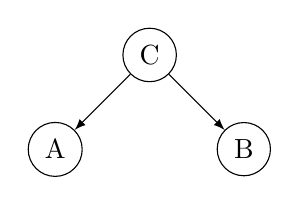
\begin{tikzpicture}[
  node distance=1cm and 0cm,
  mynode/.style={draw,circle,align=center}
]
\node[mynode] (C) {C};
\node[mynode,below left=1cm of C] (A) {A};
\node[mynode,below right=1cm of C] (B) {B};
\path (C) edge[-latex] (A)
(C) edge[-latex] (B);
\end{tikzpicture}
\caption{Conditional independence}
\label{ref:condindependence1}
\end{figure}


As seen in Figure~\ref{ref:condindependence1}, $A$ and $B$ are conditionally independent, given $C$:
\begin{definition}
$P(A,B\vert C) = P(A\vert C)P(B\vert C)$
\end{definition}

\begin{definition}
$P(A\vert B,C) = P(A\vert C)$ and $P(B\vert A,C) = P(B\vert C)$
\end{definition}

$A\independent B \vert C \neq A\independent B$
\\

As seen in Figure~\ref{ref:condindependence2}, $A\independent B$ when $C$ is unknown. When $C$ is known, $A$ and $B$ are dependent. Therefore, independence does not imply conditional independence.


\begin{figure}[h!]
\centering
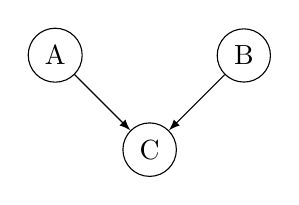
\begin{tikzpicture}[
  node distance=1cm and 1cm,
  mynode/.style={draw,circle,align=center}
]
\node[mynode] (C) {C};
\node[mynode,above left=1cm of C] (A) {A};
\node[mynode,above right=1cm of C] (B) {B};
\path (A) edge[-latex] (C)
(B) edge[-latex] (C);
\end{tikzpicture}
\caption{Conditional independence}
\label{ref:condindependence2}
\end{figure}


\section{Conditional probabilities}
\begin{definition}[Complement]
$P(\neg A\vert B) = 1 - P(A\vert B)$
\end{definition}

For $a$ and $b$ to be true, $b$ needs to be true and $a$ needs to be true given $b$:
\begin{definition}[Product rule]
$P(A,B) =P(A\vert B)P(B)$
\end{definition}

\subsection{Total probability}
\begin{definition}
$P(A) = \sum_{b\in B}{P(A,b)} = \sum_{b\in B}{P(A\vert b)P(b)}$
\end{definition}

\begin{definition}[For conditional variables]
$P(A\vert C) = \sum_{b\in B}{P(A\vert C,b)P(b\vert C)}$
\end{definition}

\subsection{Bayes' rule}
Applying product rule and total probability:
\begin{definition}
$P(A\vert B) = \frac{P(B\vert A)P(A)}{\sum_{a\in A}{P(B\vert a)P(a)}} = \frac{P(B\vert A)P(A)}{P(B)}$
\end{definition}

The terminology is: $Posterior = \frac{Prior\times Likelihood}{Normalizer}$\\

The normalizer might be difficult to calculate. It can be substituted with pseudo probabilities:
\begin{enumerate}
\item $P'(A\vert B) = P(B\vert A)P(A)$ and $P'(\neg A\vert B) = P(B\vert \neg A)P(\neg A)$
\item $P(A\vert B) = \alpha P'(A\vert B)$ and $P(\neg A\vert B) = \alpha P'(\neg A\vert B)$ with $\alpha = \frac{1}{P'(A\vert B) + P'(\neg A\vert B)}$
\end{enumerate}

\begin{definition}[General Bayes' rule]
$P(A\vert B,e) = \frac{P(B\vert A,e)P(A\vert e)}{P(B\vert e)}$
\end{definition}


\section{Bayes networks}
Bayes networks define probability distributions over random variables and allow compact specification of full joint distributions. The joint probability of the network shown in Figure~\ref{ref:samplenetwork} is: $P(A,B,C,D,E)=P(A)(B)P(C\vert A,B)P(D\vert C)P(E\vert C)$. The general equation is:
\begin{definition}
$P(x_1,...,x_n) = \prod_{i=1}^{n}{P(x_i\vert parents(X_i))}$
\end{definition}


\begin{figure}[h!]
\centering
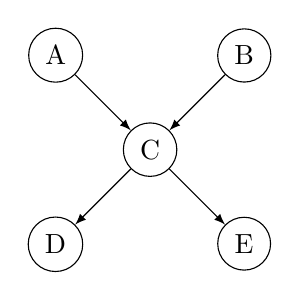
\begin{tikzpicture}[
  node distance=1cm and 1cm,
  mynode/.style={draw,circle,align=center}
]
\node[mynode] (C) {C};
\node[mynode,above left=1cm of C] (A) {A};
\node[mynode,above right=1cm of C] (B) {B};
\node[mynode,below left=1cm of C] (D) {D};
\node[mynode,below right=1cm of C] (E) {E};
\path (A) edge[-latex] (C)
(B) edge[-latex] (C)
(C) edge[-latex] (D)
(C) edge[-latex] (E);
\end{tikzpicture}
\caption{Sample Bayes network}
\label{ref:samplenetwork}
\end{figure}

\subsection{d-separation}
Stands for direction-dependent separation. d-separated variables are independent. $X$ and $Y$ are d-separated if there is no active path between them. Paths consists of {\bf triplets} as defined in Table~\ref{ref:triplets}. An inactive triplet makes an entire path inactive.

\begin{table}[h!]
\begin{center}
\begin{tabular}{|c|c|}
\hline
Active & Inactive \\
\hline
\hline
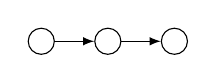
\begin{tikzpicture}[
  node distance=1cm and 1cm,
  mynode/.style={draw,circle,align=center}
]
\node[mynode] (A) {};
\node[mynode, right=0.5cm of A] (B) {};
\node[mynode, right=0.5cm of B] (C) {};
\path (A) edge[-latex] (B)
(B) edge[-latex] (C);
\end{tikzpicture}
causal chain
&
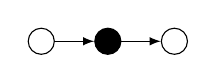
\begin{tikzpicture}[
  node distance=1cm and 1cm,
  mynode/.style={draw,circle,align=center}
]
\node[mynode] (A) {};
\node[mynode, right=0.5cm of A, fill=black] (B) {};
\node[mynode, right=0.5cm of B] (C) {};
\path (A) edge[-latex] (B)
(B) edge[-latex] (C);
\end{tikzpicture}
\\
\hline
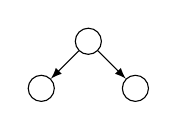
\begin{tikzpicture}[
  node distance=1cm and 1cm,
  mynode/.style={draw,circle,align=center}
]
\node[mynode] (C) {};
\node[mynode,below left=0.5cm of C] (A) {};
\node[mynode,below right=0.5cm of C] (B) {};
\path (C) edge[-latex] (A)
(C) edge[-latex] (B);
\end{tikzpicture}
common cause
&
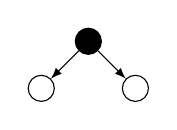
\begin{tikzpicture}[
  node distance=1cm and 1cm,
  mynode/.style={draw,circle,align=center}
]
\node[mynode, fill=black] (C) {};
\node[mynode,below left=0.5cm of C] (A) {};
\node[mynode,below right=0.5cm of C] (B) {};
\path (C) edge[-latex] (A)
(C) edge[-latex] (B);
\end{tikzpicture}
\\
\hline
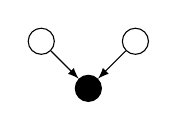
\begin{tikzpicture}[
  node distance=1cm and 1cm,
  mynode/.style={draw,circle,align=center}
]
\node[mynode,fill=black] (C) {};
\node[mynode,above left=0.5cm of C] (A) {};
\node[mynode,above right=0.5cm of C] (B) {};
\path (A) edge[-latex] (C)
(B) edge[-latex] (C);
\end{tikzpicture}
common effect
&
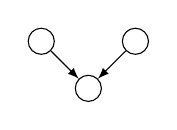
\begin{tikzpicture}[
  node distance=1cm and 1cm,
  mynode/.style={draw,circle,align=center}
]
\node[mynode] (C) {};
\node[mynode,above left=0.5cm of C] (A) {};
\node[mynode,above right=0.5cm of C] (B) {};
\path (A) edge[-latex] (C)
(B) edge[-latex] (C);
\end{tikzpicture}
\\
\hline
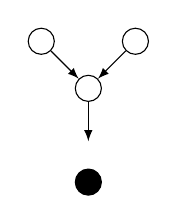
\begin{tikzpicture}[
  node distance=1cm and 1cm,
  mynode/.style={draw,circle,align=center}
]
\node[mynode] (C) {};
\node[mynode,above left=0.5cm of C] (A) {};
\node[mynode,above right=0.5cm of C] (B) {};
\node[mynode,below=0.5cm of C,color=white] (D) {};
\node[mynode,below=0cm of D, fill=black] (E) {};
\path (A) edge[-latex] (C)
(B) edge[-latex] (C)
(C) edge[-latex] (D);
\end{tikzpicture}
&
\\
\hline
\end{tabular}
\end{center}
\caption{Active and inactive triplets with known variables filled}
\label{ref:triplets}
\end{table}


\chapter{Problem Solving}
\section{Introduction}
A {\bf problem solving agent} requires a deterministic and fully observable environment. Please see Chapter~\ref{ref:chapterplanning} for planning in more complex environments. Table~\ref{ref:search} compares general search algorithms.

\begin{table}[h!]
\begin{center}
\begin{tabular}{|l||c|c|c|}
\hline
 & Breadth-first & Uniform-cost & Depth-first\\
\hline
\hline
Expansion order
&
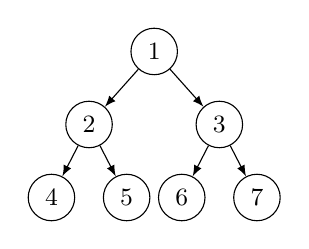
\begin{tikzpicture}[
  node distance=1cm and 1cm,
  mynode/.style={draw,circle,align=center},
  font=\small
]
\node[mynode] (A) {1};
\node[mynode,below left=0.5cm and 0.4 of A] (B) {2};
\node[mynode,below right=0.5cm and 0.4 of A] (C) {3};
\node[mynode,below left=0.5cm and 0.05 of B] (D) {4};
\node[mynode,below right=0.5cm and 0.05 of B] (E) {5};
\node[mynode,below left=0.5cm and 0.05 of C] (F) {6};
\node[mynode,below right=0.5cm and 0.05 of C] (G) {7};
\path (A) edge[-latex] (B)
(A) edge[-latex] (C)
(B) edge[-latex] (D)
(B) edge[-latex] (E)
(C) edge[-latex] (F)
(C) edge[-latex] (G);
\end{tikzpicture}
&
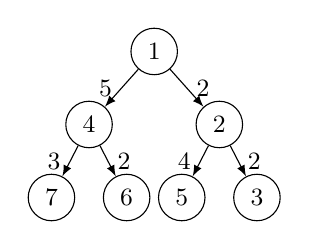
\begin{tikzpicture}[
  node distance=1cm and 1cm,
  mynode/.style={draw,circle,align=center},
  font=\small
]
\node[mynode] (A) {1};
\node[mynode,below left=0.5cm and 0.4 of A] (B) {4};
\node[mynode,below right=0.5cm and 0.4 of A] (C) {2};
\node[mynode,below left=0.5cm and 0.05 of B] (D) {7};
\node[mynode,below right=0.5cm and 0.05 of B] (E) {6};
\node[mynode,below left=0.5cm and 0.05 of C] (F) {5};
\node[mynode,below right=0.5cm and 0.05 of C] (G) {3};
\path (A) edge[-latex] node[left] {5} (B)
(A) edge[-latex] node[right] {2} (C)
(B) edge[-latex] node[left] {3} (D)
(B) edge[-latex] node[right] {2} (E)
(C) edge[-latex] node[left] {4} (F)
(C) edge[-latex] node[right] {2} (G);
\end{tikzpicture}
&
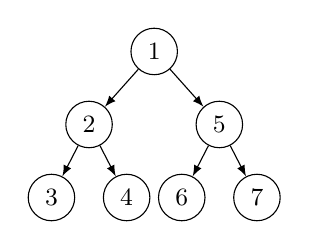
\begin{tikzpicture}[
  node distance=1cm and 1cm,
  mynode/.style={draw,circle,align=center},
  font=\small
]
\node[mynode] (A) {1};
\node[mynode,below left=0.5cm and 0.4 of A] (B) {2};
\node[mynode,below right=0.5cm and 0.4 of A] (C) {5};
\node[mynode,below left=0.5cm and 0.05 of B] (D) {3};
\node[mynode,below right=0.5cm and 0.05 of B] (E) {4};
\node[mynode,below left=0.5cm and 0.05 of C] (F) {6};
\node[mynode,below right=0.5cm and 0.05 of C] (G) {7};
\path (A) edge[-latex] (B)
(A) edge[-latex] (C)
(B) edge[-latex] (D)
(B) edge[-latex] (E)
(C) edge[-latex] (F)
(C) edge[-latex] (G);
\end{tikzpicture}
\\
\hline
Expansion strategy & shallowest & cheapest & deepest\\
\hline
Optimal & yes & yes & no\\
\hline
Complete & yes & yes & no\\
\hline
Frontier size ($n$ levels) & $2n$ & $2n$ & $n$\\
\hline
\end{tabular}
\end{center}
\caption{Comparison of search algorithms}
\label{ref:search}
\end{table}

\section{A* search}
$A*$ expands the path with that has the minimum value $f$.

\begin{definition}[A* cost function]
$f = g + h$ with $g(path) =$ current path cost and $h(path) = h(s) =$ estimated distance to goal
\end{definition}

$f$ is a {\bf heuristic function}. $A*$ finds lowest cost path if: $h(s) <$ true cost. Subsequently, $h$ never overestimates and is optimistic/admissible. See Figure~\ref{ref:heuristic} for an example.

\begin{figure}[h!]
\centering
\begin{subfigure}[b]{0.3\textwidth}
\begin{tabular}{|c|c|c|c|c|c|}
\hline
S &\cellcolor{black}&&&& \\
\hline
&\cellcolor{black}&&&& \\
\hline
&\cellcolor{black}&&&& \\
\hline
&\cellcolor{black}&&&& \\
\hline
&&&&&G \\
\hline
\end{tabular}
\end{subfigure}
\begin{subfigure}[b]{0.3\textwidth}
\begin{tabular}{|c|c|c|c|c|c|}
\hline
9&8&7&6&5&4 \\
\hline
8&7&6&5&4&3 \\
\hline
7&6&5&4&3&2 \\
\hline
6&5&4&3&2&1 \\
\hline
5&4&3&2&1&0 \\
\hline
\end{tabular}
\end{subfigure}
\caption{Sample world and heuristic}
\label{ref:heuristic}
\end{figure}


\section{Policy}
A {\bf policy} specifies what an agent should do for any state that the agent might reach. An {\bf optimal policy} is a policy that yields the highest expected {\bf utility} (meaning "the quality of being useful"). See Figure~\ref{ref:policy} for an example.

\begin{figure}[h!]
\centering
\begin{subfigure}[b]{0.3\textwidth}
\begin{tabular}{|c|c|c|c|c|c|}
\hline
&\cellcolor{black}&&&& \\
\hline
&\cellcolor{black}&&&& \\
\hline
&\cellcolor{black}&&&& \\
\hline
&\cellcolor{black}&&&& \\
\hline
&&&&\cellcolor{black}&G \\
\hline
\end{tabular}
\end{subfigure}
\begin{subfigure}[b]{0.3\textwidth}
\begin{tabular}{|c|c|c|c|c|c|}
\hline
$\downarrow$&&$\rightarrow$&$\rightarrow$&$\rightarrow$&$\downarrow$ \\
\hline
$\downarrow$&&$\rightarrow$&$\rightarrow$&$\rightarrow$&$\downarrow$ \\
\hline
$\downarrow$&&$\rightarrow$&$\rightarrow$&$\rightarrow$&$\downarrow$ \\
\hline
$\downarrow$&&$\rightarrow$&$\rightarrow$&$\rightarrow$&$\downarrow$ \\
\hline
$\rightarrow$&$\rightarrow$&$\uparrow$&$\uparrow$&&* \\
\hline
\end{tabular}
\end{subfigure}
\caption{Sample world and policy}
\label{ref:policy}
\end{figure}


\chapter{Logic}
\section{Introduction}

\begin{table}[h!]
\begin{center}
\begin{tabular}{|l|c|c|}
\hline
& World & Beliefs \\
\hline
\hline
Probability theory & facts & $[0,1]$ \\
\hline
Propositional logic & facts & true, false, unknown \\
\hline
First-order logic & relations, objects, functions & true, false, unknown \\
\hline
\end{tabular}
\end{center}
\caption{Comparison of formal languages}
\label{ref:complang}
\end{table}


\section{Propositional logic}
Equivalent to Boolean Algebra. There are efficient inference algorithms to determine validity and satisfiability. Limitations:
\begin{itemize}
  \item It can only handle true and false values
  \item No capability to handle uncertainty
  \item No objects
  \item No shortcuts to express similar properties, only like: $A_1 \wedge A_2 \wedge ... \wedge A_n$
\end{itemize}


\section{First-order logic}
First-order logic is sufficiently expressive to represent a reasonable amount of our commonsense knowledge. It is also used in many further representation languages and has been studied intensively for many decades. The first-order logic syntax is defined in Figure~\ref{ref:firstordersyntax}.

\begin{figure}[h!]
\centering
\begin{tabular}{lcl}
$Sentence$ & $\rightarrow$ & $AtomicSentence$ $\vert$ $ComplexSentence$ \\
$AtomicSentence$ & $\rightarrow$ & $Predicate$ $\vert$ $Predicate(Term,...)$ $\vert$ $Term=Term$ \\
$ComplexSentence$ & $\rightarrow$ & $(Sentence)$ $\vert$ $[Sentence]$ \\
 & $\vert$ & $\neg Sentence$ \\
 & $\vert$ & $Sentence \wedge Sentence$ \\
 & $\vert$ & $Sentence \vee Sentence$ \\
 & $\vert$ & $Sentence \implies Sentence$ \\
 & $\vert$ & $Sentence \iff Sentence$ \\
 & $\vert$ & $Quantifier$ $Variable, ...$ $Sentence$ \\
\\
$Term$ & $\rightarrow$ & $Function(Term,...)$ \\
 & $\vert$ & $Constant$ \\
 & $\vert$ & $Variable$ \\
 \\
$Quantifier$ & $\rightarrow$ & $\forall$ $\vert$ $\exists$ \\
$Constant$ & $\rightarrow$ & $A$ $\vert$ $X_1$ $\vert$ $John$ $\vert$ $...$ \\
$Variable$ & $\rightarrow$ & $a$ $\vert$ $x$ $\vert$ $s$ $\vert$ $..$ \\
$Predicate$ & $\rightarrow$ & $True$ $\vert$ $False$ $\vert$ $After$ $\vert$ $Loves$ $\vert$ $Raining$ $\vert$ $...$\\
$Function$ & $\rightarrow$ & $FullName$ $\vert$ $PhoneNumber$ $\vert$ $...$ \\
\\
$OPERATOR$ $PRECEDENCE$ & $:$ & $\neg,=,\wedge,\vee,\implies,\iff$ \\
\end{tabular}
\caption{First-order logic syntax}
\label{ref:firstordersyntax}
\end{figure}



\section{Higher-order logic}
Views relations and functions as objects themselves. Therefore, it allows more powerful expressions, e.g. relations on relations: $\forall_R$ $Transitive(R)\iff \forall a,b,c$ $R(a,b)\wedge R(b,c) \implies R(a,c)$


\chapter{Planning}
\label{ref:chapterplanning}
A {\bf planning agent} interleaves planning and execution. This is necessary for environments which are {\bf stochastic}, {\bf multi agent}, {\bf partially observable} or {\bf unknown}. Plans might be {\bf hierarchical} which consist of actions on different levels. Some of these levels can be planned ahead, others while executing the plan. Example: A* can find a route from A to Z but the route might change due to accidents. Low-level actions such as turning the steering wheel or pressing the pedals cannot be planned well-ahead in time in the real world.


\chapter{Learning}

{\bf Machine learning} is the field of study that gives computers the ability to learn without being explicitly programmed.

What:
\begin{itemize}
  \item Parameters
  \item Structure
  \item Hidden concepts
\end{itemize}

What from:
\begin{itemize}
  \item Supervised
  \item Unsupervised
  \item Reinforcement
\end{itemize}

What for:
\begin{itemize}
  \item Prediction
  \item Diagnostics
  \item Summarization
  \item ...
\end{itemize}

How:
\begin{itemize}
  \item Passive: learning agent is just an observer and has no impact on the data itself
  \item Active
  \item Online: learning while data is being generated
  \item Offline: learning by processing data in batch
\end{itemize}

Outputs:
\begin{itemize}
  \item Classification: discrete values
  \item Regression: continuous
\end{itemize}

Details:
\begin{itemize}
  \item Generative: model data as generally as possible
  \item Descriminative: seek to distinguish data
\end{itemize}


\chapter{Supervised learning}
Supervised learning learns from training examples. If there are not sufficiently enough tfeatures, the learning algorithm may {\bf underfit}. In contrast, it may {\bf overfit} for too many features meaning it only matches the training data well but fails to generalize to new examples.

\section{Linear regression}
{\bf Linear regression} computes a linear regression function for $m$ {\bf training examples} having $n$ {\bf features}. The objective is to minimize the cost function:
\begin{definition}[Cost function]
$J(\theta) = \frac{1}{2m}\sum_{i=1}^m(h_\theta(x^{(i)})-y^{(i)})^2$
\end{definition}

Where the hypothesis $h_\theta(x^{(i)})$ is given by the linear model:
\begin{definition}[Hypothesis]
$h_\theta(x^{(i)}) = \theta^{T}x = \theta_0 x_0 + \theta_1 x_1 + ... + \theta_n x_n$ with $x_0 = 1$
\end{definition}

The parameters of the model to be learned are the $\theta_j$ values. One way to do this is to use the batch {\bf gradient descent} algorithm. Through is step, the parameters $\theta_j$ come closer to the optimal values that will achieve the lowest cost $J(\theta)$. If the {\bf learning rate} $\alpha$ is too large, gradient descent might not converge and overshoot the minimum after a certain amount of iterations. Gradient descent might generally not find the global but the local minimum. Gradient descent returns the global minimum for convex or bowl-shaped cost functions which do not have local optima. {\bf Feature normalization} allows to perform gradient descent quickly by scaling each feature.


\begin{definition}[Gradient descent] ~\\
loop until converge \{ \\
$\theta_j := \theta_j - \alpha \frac{1}{m}\sum_{i=1}^m(h_\theta(x^{(i)})-y^{(i)})x_j^{(i)}$ (simultaneously update $\theta_j$ for all $j$) \\
\}
\end{definition}

\begin{definition}[Feature normalization]
$x_j' = \frac{x_j - \mu_j}{\sigma_j}$
\end{definition}

{\bf Vectorization} allows to do the updates simultaneously through various matrix operations. Matrix multiplications can be executed very efficiently (Strassen algorithm). Matrix $X$ contains $m$ training data rows and $n$ features where row $x_0$ contains entirely 1s. The cost function and gradient descent then look:

\begin{definition}[Vectorized cost function] ~\\
$J(\theta) = \frac{1}{2m}(X\theta-y)^T(X\theta-y)$\\
\end{definition}

\begin{definition}[Vectorized gradient descent] ~\\
$\theta := \theta - \alpha \frac{1}{m}X^{T}(h_{\theta}(x)-y) := \theta - \alpha \frac{1}{m}X^{T}(X\theta-y)$
\end{definition}

The {\bf normal equation} is a closed-form solution for linear regression which requires no loop, no learning rate and no feature normalization. It may be too slow for very large matrices as inversion is $O(n^3)$. $X$ may be singular and cannot be inverted. It is usually recommended to calculate the pseudo inverse.
\begin{definition}[Normal equation]
$\theta = (X^{T}X)^{-1}X^{T}y$
\end{definition}


\section{Logistic regression}

Logistic regression allows linear classification. The parameters $\theta_j$ comprise the linear separator called decision boundary. The hypothesis is defined as:
\begin{definition}[Hypothesis]
$h_\theta(x) = g(\theta^{T}x)$
\end{definition}

The hypothesis can be more complex to use logistic regression for non-linear classification. $g$ is the {\bf sigmoid function} which is defined as:
\begin{definition}[Sigmoid function]
$g(z) = \frac{1}{1 + e^{-z}}$
\end{definition}

The cost function in logistic regression is convex:
\begin{definition}[Cost function] ~\\
$J(\theta) = \frac{1}{m}\sum_{i=1}^m[-y^{(i)}log(h_{\theta}(x^{(i)}))-(1-y^{(i)})log(1-h_{\theta}(x^{(i)}))]$
\end{definition}

\begin{definition}[Vectorized cost function] ~\\
$J(\theta) = \frac{1}{m}[-y^T log(g(X\theta))-(1-y)^T log(1-g(X\theta))]$
\end{definition}

This gradient descent looks identical to the linear regression gradient but the formula is actually different because of the different definition of $h_{\theta}(x)$.
\begin{definition}[Gradient descent]
$\theta_j := \theta_j - \alpha \frac{1}{m}\sum_{i=1}^m(h_\theta(x^{(i)})-y^{(i)})x_j^{(i)}$
\end{definition}

\begin{definition}[Vectorized gradient descent] ~\\
$\theta := \theta - \alpha \frac{1}{m}X^{T}(g(X\theta)-y)$
\end{definition}


\section{Regularization}
{\bf Regularization} allows to prevent overfitting by "penalizing" large $\theta_j$ values. Feature $x_0$ is usually not affected by regularization. If $\lambda$ is set too large, the learning algorithm may underfit. For linear regression, the definitions change to:

\begin{definition}[Regularized linear regression cost function] ~\\
$J(\theta) = \frac{1}{2m}[\sum_{i=1}^m(h_\theta(x^{(i)})-y^{(i)})^2+ {\bf \lambda \sum_{j=1}^n\theta_j^2}]$
\end{definition}

\begin{definition}[Regularized linear regression gradient descent] ~\\
$\theta_j := \theta_j - \alpha[ \frac{1}{m}\sum_{i=1}^m(h_\theta(x^{(i)})-y^{(i)})x_j^{(i)} {\bf +\frac{\lambda}{m}\theta_j}]$
\end{definition}

Regularization also allows the normal equation to be invertible by adding a $(n+1)\times (n+1)$ matrix:
\begin{definition}[Regularized normal equation] ~\\
$\theta = (X^{T}X+\lambda
\begin{pmatrix}
0 & & & \\
&1& &\\
& & ... & \\
& & & 1
\end{pmatrix}
)^{-1}X^{T}y$
\end{definition}

For logistic regression, the definitions change to:

\begin{definition}[Regularized logistic regression cost function] ~\\
$J(\theta) = \frac{1}{m}\sum_{i=1}^m[-y^{(i)}log(h_{\theta}(x^{(i)}))-(1-y^{(i)})log(1-h_{\theta}(x^{(i)}))] {\bf + \frac{\lambda}{2m}\sum_{j=1}^n\theta_j^2}$
\end{definition}

\begin{definition}[Regularized logistic regression gradient descent] ~\\
$\theta_j := \theta_j - \alpha[ \frac{1}{m}\sum_{i=1}^m((h_\theta(x^{(i)})-y^{(i)})x_j^{(i)} ) {\bf + \frac{\lambda}{m}\theta_j}]$
\end{definition}


\section{Neural network}
A neuron has {\bf inputs} and an {\bf output} as seen in Figure~\ref{ref:neuron}. A {\bf neural network} consists of layers of {\bf neurons}. Each layer has a {\bf bias term} of value 1. The parameters $\theta_j$ are called {\bf weights} in some sources. The hypothesis is called {\bf Sigmoid activation function}.

\begin{figure}[h!]
\centering
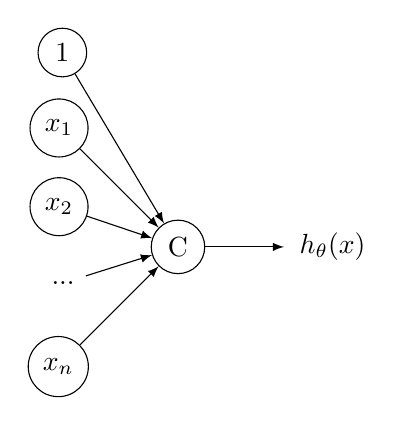
\begin{tikzpicture}[
  node distance=1cm and 1cm,
  mynode/.style={draw,circle,align=center}
]
\node[mynode] (C) {C};
\node[mynode,above left=2cm and 1cm of C] (X0) {$1$};
\node[mynode,above left=1cm and 1cm of C] (X1) {$x_1$};
\node[mynode,above left=0cm and 1cm of C] (X2) {$x_2$};
\node[mynode,below left=0cm and 1cm of C,draw=white] (X3) {...};
\node[mynode,below left=1cm and 1cm of C] (XN) {$x_n$};
\node[mynode,right=1cm and 1cm of C,draw=white] (h) {$h_{\theta}(x)$};
\path (X0) edge[-latex] (C)
(X1) edge[-latex] (C)
(X2) edge[-latex] (C)
(X3) edge[-latex] (C)
(XN) edge[-latex] (C)
(C) edge[-latex] (h);
\end{tikzpicture}
\caption{Neuron with bias term $x_0=1$}
\label{ref:neuron}
\end{figure}

\begin{definition}[Sigmoid activation function]
$h_\theta(x) = \frac{1}{1+e^{-\theta^{T}x}}$
\end{definition}

Each neural network has an {\bf input layer}, $\ge 0$ {\bf hidden layers} and an {\bf output layer} as seen in Figure~\ref{ref:neuralnetwork}. The value $a_i^{(j)}$ is called {\bf activation} or {\bf forward propagation} of unit $i$ in layer $j$. $\Theta^{(j)}$ is a matrix of weights to map from layer $j$ to layer $j+1$. If network has $s_j$ units in layer $j$, $s_{j+1}$ units in layer $j+1$, then $\Theta^{(j)}$ will be of dimension $s_{j+1}\times (s_j + 1)$. For the neural network in Figure~\ref{ref:neuralnetwork}, the mapping is defined in Figure~\ref{ref:neuralnetworkmapping}. \\

The cost function for $K$ output units and $L$ layers is defined as follows (with $h_\Theta(x) \in \mathbb{R}^K$ and $(h_\Theta(x))_i = i^{th}$ output):

\begin{definition}[Regularized cost function] ~\\
$J(\Theta) = -\frac{1}{m}[\sum_{i=1}^m \sum_{k=1}^K y_k^{(i)}log(h_{\Theta}(x^{(i)}))_k+(1-y_k^{(i)})log(1-h_{\Theta}(x^{(i)}))_k] \\
+ \frac{\lambda}{2m}\sum_{l=1}^{L-1}\sum_{i=1}^{s_{l}}\sum_{j=1}^{s_{l+1}}(\Theta_{ij}^{(l)})^2$
\end{definition}

\begin{figure}[h!]
\centering
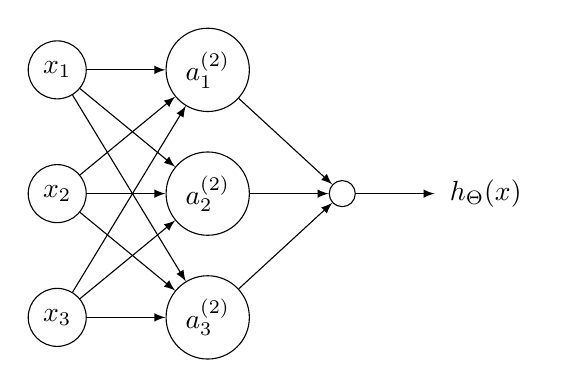
\begin{tikzpicture}[
  node distance=1cm and 1cm,
  mynode/.style={draw,circle,align=center}
]
\node[mynode] (A12) {$a_1^{(2)}$};
\node[mynode,below=0.5cm of A12] (A22) {$a_2^{(2)}$};
\node[mynode,below=0.5cm of A22] (A32) {$a_3^{(2)}$};
\node[mynode,left=0cm and 1cm of A12] (X1) {$x_1$};
\node[mynode,left=0cm and 1cm of A22] (X2) {$x_2$};
\node[mynode,left=0cm and 1cm of A32] (X3) {$x_3$};
\node[mynode,right=0cm and 1cm of A22] (L3) {};
\node[mynode,right=0cm and 1cm of L3,draw=white] (h) {$h_{\Theta}(x)$};
\path (X1) edge[-latex] (A12)
(X1) edge[-latex] (A22)
(X1) edge[-latex] (A32)
(X2) edge[-latex] (A12)
(X2) edge[-latex] (A22)
(X2) edge[-latex] (A32)
(X3) edge[-latex] (A12)
(X3) edge[-latex] (A22)
(X3) edge[-latex] (A32)
(A12) edge[-latex] (L3)
(A22) edge[-latex] (L3)
(A32) edge[-latex] (L3)
(L3) edge[-latex] (h);
\end{tikzpicture}
\caption{Neural network with three layers (bias terms not displayed)}
\label{ref:neuralnetwork}
\end{figure}

\begin{figure}[h!]
\centering
\begin{tabular}{lcl}
$a_1^{(2)}$ & $=$ & $g(\Theta_{10}^{(1)}x_0 + \Theta_{11}^{(1)}x_1 + \Theta_{12}^{(1)}x_2 + \Theta_{13}^{(1)}x_3)$ \\
$a_2^{(2)}$ & $=$ & $g(\Theta_{20}^{(1)}x_0 + \Theta_{21}^{(1)}x_1 + \Theta_{22}^{(1)}x_2 + \Theta_{23}^{(1)}x_3)$ \\
$a_3^{(2)}$ & $=$ & $g(\Theta_{30}^{(1)}x_0 + \Theta_{31}^{(1)}x_1 + \Theta_{32}^{(1)}x_2 + \Theta_{33}^{(1)}x_3)$ \\
$h_{\Theta}(x)$ & $=$ & $a_1^{(3)}$ $=$ $g(\Theta_{10}^{(2)}a_0^{(2)} + \Theta_{11}^{(2)}a_1^{(2)} + \Theta_{12}^{(2)}a_2^{(2)} + \Theta_{13}^{(2)}a_3^{(2)})$ \\
\end{tabular}
\caption{Activation of layers in a neural network}
\label{ref:neuralnetworkmapping}
\end{figure}

\subsection{Backpropagation}
Training a neural network requires to $\min\limits_{\Theta}J(\Theta)$, e.g. through gradient descent which requires $J(\Theta)$ and $\frac{\partial}{\partial \Theta_{ij}^{(l)}}J(\Theta)$. {\bf Backpropagation} is a method to compute the gradient as described in Figure~\ref{ref:backpropagation}. This algorithm can also be vectorized. The derivative of the Sigmoid function is defined as follows:
\begin{definition}[Derivative of Sigmoid function] ~\\
$g^{'}(x)=g(x)*(1-g(x))$
\end{definition}

\begin{figure}[h!]
Training set $\{(x^{(1)},y^{(1)}),...,(x^{(m)},y^{(m)})\}$ \\
Set $\Delta_{ij}^{(l)}=0$ (for all $l,i,j$). \\
For $i=1$ to $m$
\begin{tabbing}
~~~~ \= Set $a^{(i)}=x^{(i)}$ \\
\> Perform forward propagation to compute $a^{(l)}$ for $l=2,3,...,L$ \\
\> Using $y^{(i)}$, compute $\delta^{(L)}=a^{(L)}-y^{(i)}$ ("error") \\
\> Compute $\delta^{(L-1)},\delta^{(L-2)},...,\delta^{(2)}$, e.g. $\delta^{(2)}=(\Theta^{(2)})^T\delta^{(3)}.*g^{'}(z^{(2)})$ (element-wise multiplication) \\
\> $\Delta_{ij}^{(l)}:=\Delta_{ij}^{(l)}+a_j^{(l)}\delta_i{(l+1)}$ \\
$D_{ij}^{(l)}:=\frac{1}{m}\Delta_{ij}^{(l)}+\lambda\Theta_{ij}^{(l)}$ if $j\ne0$ (no regularization of bias terms) \\
$D_{ij}^{(l)}:=\frac{1}{m}\Delta_{ij}^{(l)}$ if $j=0$
\\
\\
$\frac{\partial}{\partial \Theta_{ij}^{(l)}}J(\Theta)=D_{ij}^{(l)}$
\end{tabbing}
\caption{Backpropagation algorithm}
\label{ref:backpropagation}
\end{figure}

$\Theta_{ij}^{(l)}$ needs to have an initial value. If $\Theta$ was entirely 0, {\bf symmetry} would create a highly redundant neural network with poor learning capabilities. {\bf Random initialization} allows symmetry breaking by initializing each $\Theta_{ij}^{(l)}$ to a random value in $[-\epsilon,\epsilon]$

\subsection{Gradient checking}
As backpropagation is a complex algorithm, subtile bugs might not be caught and gradient descent might not reach the intended global minimum but only a more expensive minimum. {\bf Gradient checking} allows to approximate the gradient and compare it to the gradient returned by backpropagation. The approximation is computed as follows for each feature $\theta_i$:
\begin{definition}[Gradient checking] ~\\
$\frac{\partial}{\partial\theta_i}J(\theta)\approx\frac{J(...,\theta_{i-1},\theta_{i}+\epsilon,\theta_{i+1},...)+J(...,\theta_{i-1},\theta_{i}-\epsilon,\theta_{i+1},...)}{2\epsilon}$ for small $\epsilon$
\end{definition}

\chapter{Unsupervised learning}
\chapter{Reinforcement learning}

\chapter{Localization}
\section{Grid localization}
\section{Kalman filter}
\section{Particle filter}


\end{document}